\section{Introduction}

Nowadays data collection is omnipresent. However, most of the research is done on the extraction of information from large data sets (so called Big Data Analysis). Therefore small data sets collected in day-to-day practice of professionals is often overlooked. 
Clinicians and hospitals collect for example a lot of data on their patients, the used therapies and the outcomes. Unfortunately this data is often not used to inform future practice. This project aims to implement an intelligent agent that provides statistical advice on the analysis of such data. The system will be based on the design described in the related paper by Sassoon \textit{et al.} \cite{sassoon2014}.

This preliminary report first clarifies the project aims and objectives in \autoref{sub:aims}. Second, the used methodologies and the general technical specification are explained (see \autoref{sub:methodologies} and \autoref{sub:technical}). This is followed by a background research in \autoref{sec:background} providing a review of the theoretical aspects of argumentation frameworks and their extensions and the theory behind statistical model selection. A critical review of related literature and approaches is given. At the end of this preliminary report a detailed project plan is presented (see \autoref{sec:projectplan}) which depicts the planned progress of this thesis till the end of August 2016.

\subsection{Project Aims and Objectives} 
\label{sub:aims}

The aims of this project can be divided into a list or primary and secondary goals. For a successful project progression the following primary objectives have to be reached:
\begin{itemize}
	\item General explanation and summary of \glspl{AF}, \glspl{EAF} and statistical model selection.
	\item Development of an \textit{Ruby on Rails} web application that implements the requirements proposed in \cite{sassoon2014} including but not limited to:
	\begin{itemize}
		\item An approach to instantiate and solve \glspl{AF} and \glspl{EAF}.
		\item The ability to store, manage and reuse research questions, analysis, preferences for statistical models and data sets.
		\item An easy to use user interface to upload clinical data and run analyses in an interactive way using the theory proposed by Sassoon \textit{et al}.
		\item The ability to deal with preferences between models on a meta-level using \glspl{EAF} while taking into account global and personal (end user) preferences.
		\item A user rights management to allow the system to be used by clinicians and statisticians.
		\item A small set of statistical models and their assumptions integrated in the system (externally provided).
		\item A comprehensive set of unit and integration tests of the system.
		\item Hosting of this web application at a public accessible provider.
	\end{itemize}	
	\item The system should provide the end user with an explanation why a statistical model should be used, and why one model might be preferred over another one.
\end{itemize}


The secondary goals are desired to be achieved but do not influence the successful finalisation of the project. These objectives are the following:
\begin{itemize}
	\item A documentation of the developed system providing information on how to use it and an overview over the key components of the application.
	\item A reusable implementation to solve standard \glspl{AF} in Ruby as a \texttt{gem} including documentation and a comprehensive set of unit tests.
	\item A reusable implementation to solve \glspl{EAF} in Ruby as a \texttt{gem} including documentation and a comprehensive set of unit tests.
	\item Extended sets of statistical models and their assumptions.
	\item A graphical representation of the arguments explaining the actual analysis outcome of the system.
\end{itemize}


\subsection{Methodologies of the Project}
\label{sub:methodologies}
This project will be developed in an agile way. To ensure that it meets the requirements described by Sassoon \textit{et al.} (\cite{sassoon2014}, see \autoref{sub:statistical_model_selection}), the main author of that paper is treated as a client during the requirements analysis and the testing phase. For the actual development process the Use-Case 2.0 approach by Jacobson \textit{et al.} \cite{jacobson2011usecase} is used as it provides a great way to communicate, specify and iterate over functional (independent) parts of the system. Due to its descriptive nature it does not require any knowledge about the actual process to be easy understandable. The key components of this approach are Use-Cases, Use-Case Flows, Use-Case Slices and Test Cases. The later will be used for the test- and behaviour-driven development approach employed in this project. These methodologies will be explained and introduced in detail later in this thesis. 

As a project communication and management tool Trello\footnote{http://www.trello.com} is utilized as it provides an easy-to-use and interactive way of dealing with cards (in our case use-cases and tasks) and to group them. As the final application will be developed in four release cycles (RC~1 - 4, see \autoref{sec:projectplan}), track of the already achieved intermediate steps and the actual progress of the development process can be recorded efficiently. Labels and different lists visualise the status and progress of each task and use-case (see \autoref{fig:trello}).


\begin{figure}[h]
\centering
	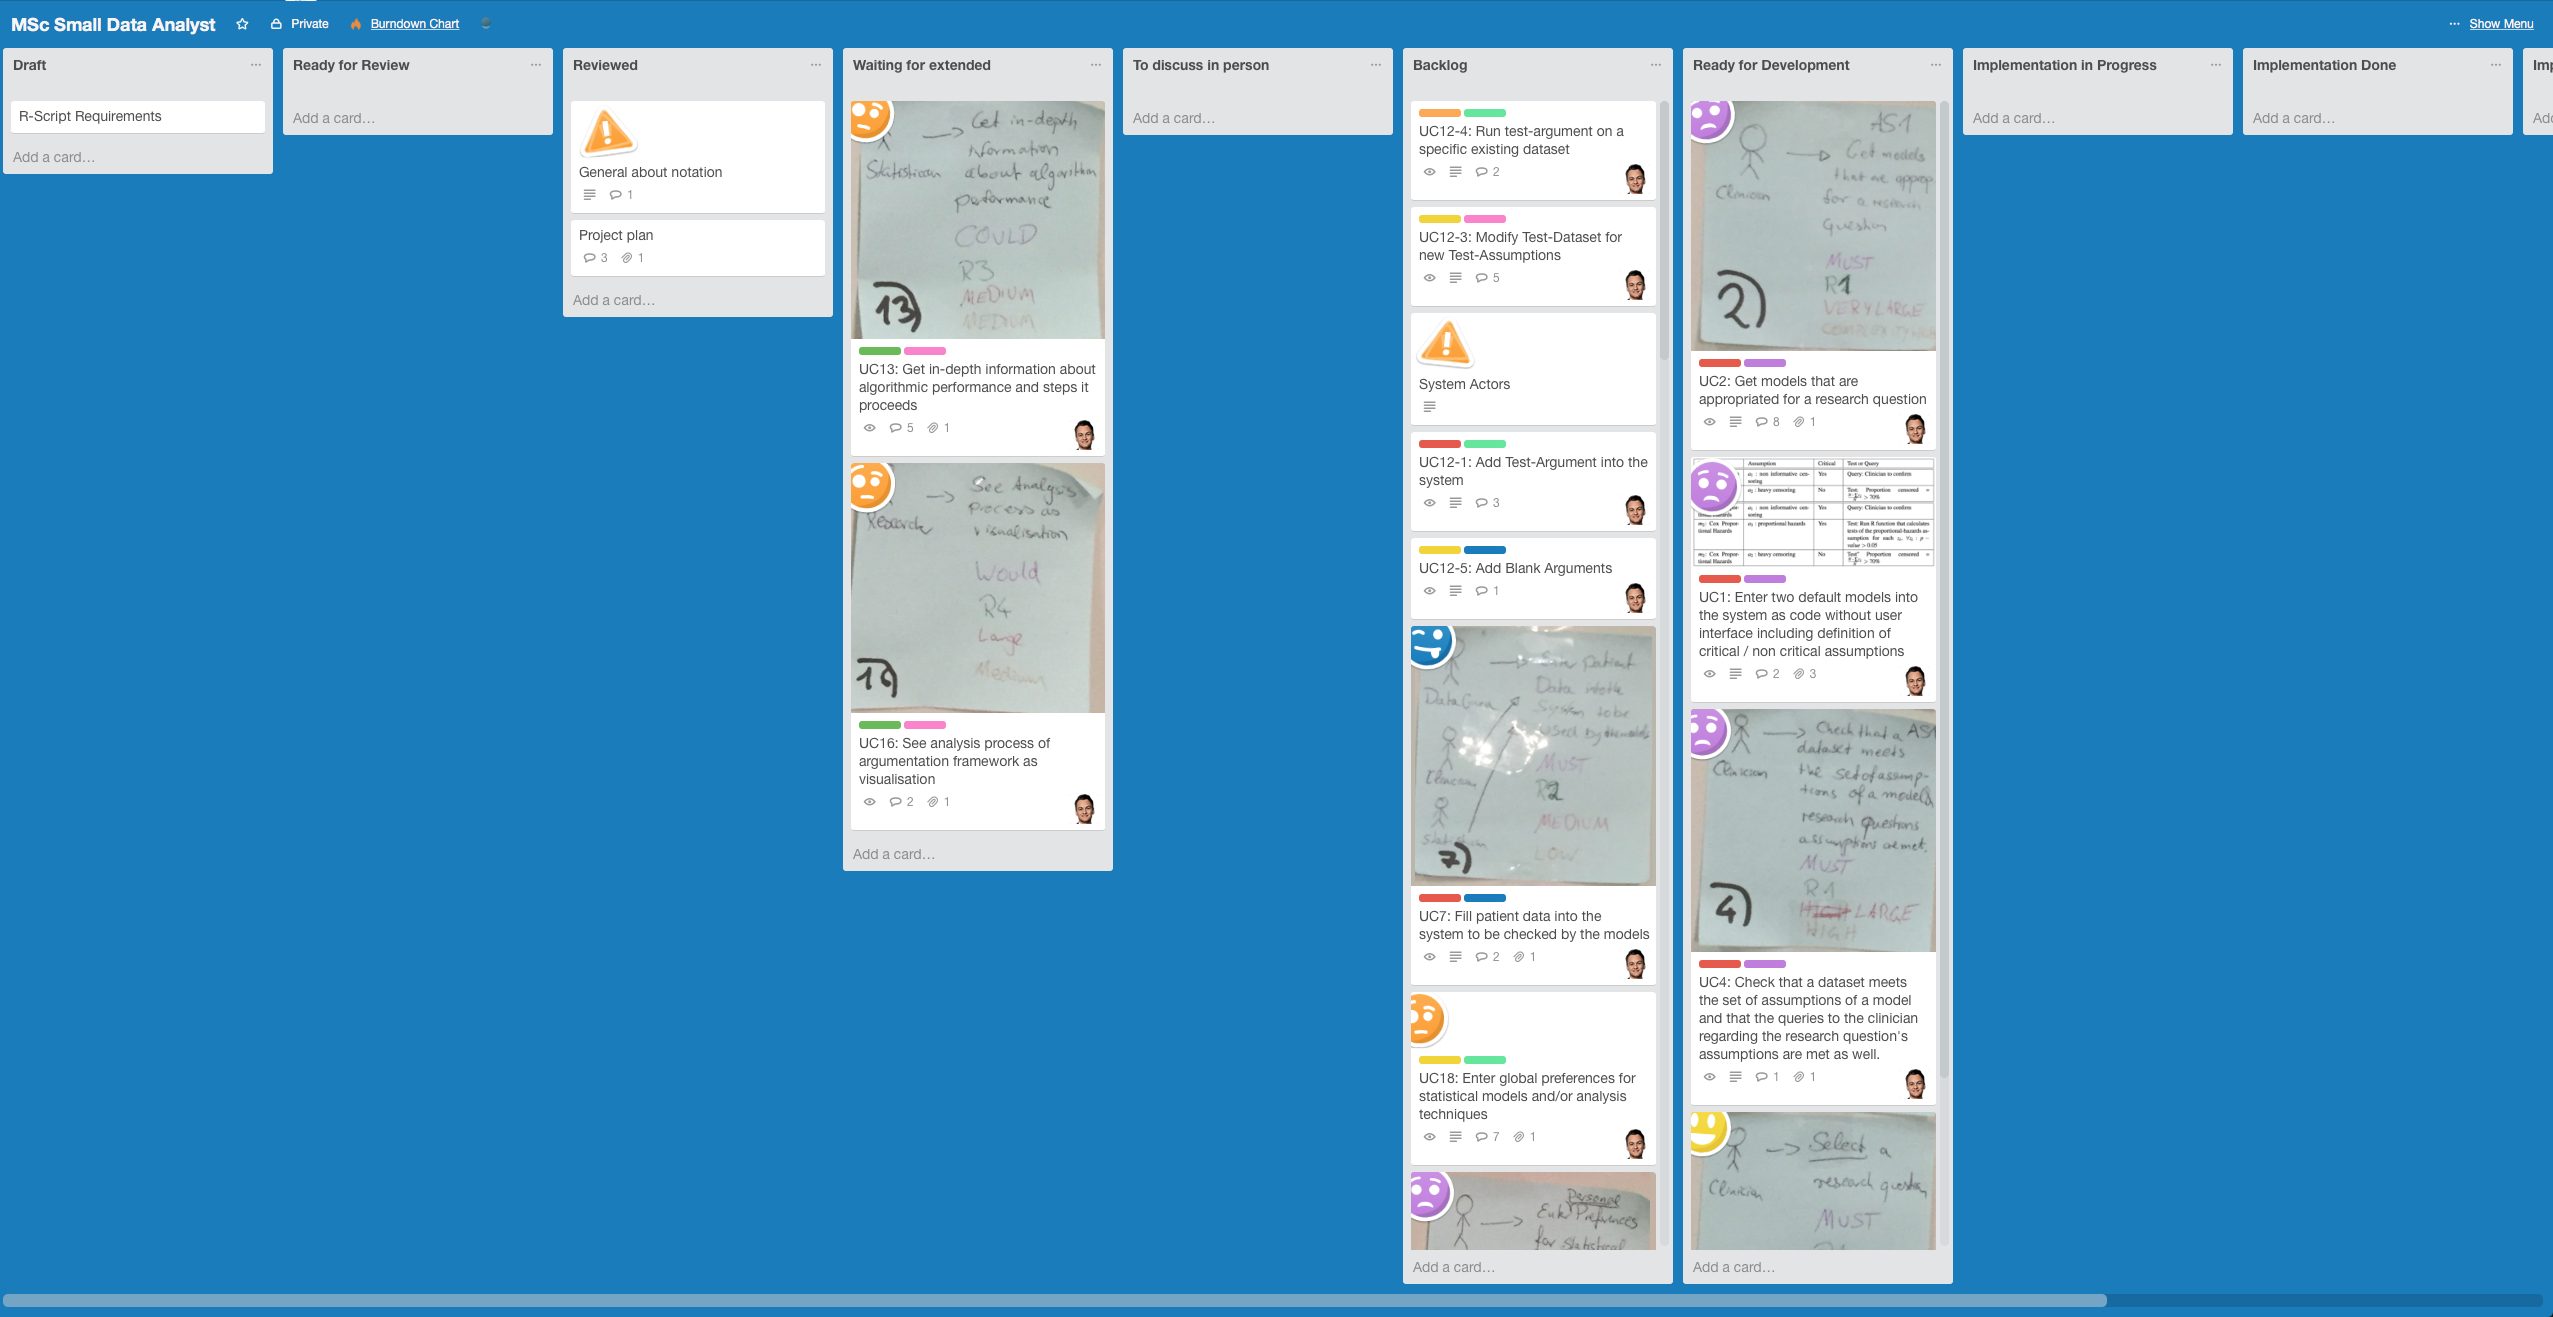
\includegraphics[page=1,width=\textwidth]{figures/trello}
\caption{Screenshot of the used Trello board used as project management tool.}
\label{fig:trello}
\end{figure}


\subsection{Technical Specification}
\label{sub:technical}

As the system should be accessible by multiple users and from different departments (e.g. clinicians and statisticians), it will be developed as a web-application in \texttt{Ruby on Rails 4}\footnote{http://rubyonrails.org} and will be hosted on \texttt{Heroku}\footnote{http://www.heroku.com}. 

The used datasets are anonymised, so data protection issues are reduced to a minimum and the datasets can be hosted in the cloud. \texttt{PostgreSQL}\footnote{http://www.postgresql.org} will be used as a database, as it is well integrated on \texttt{Heroku} and provides high scalability.

Most of the assumption tests for the statistical models will be performed in \texttt{R}, as this is a common used language for statistical calculations and well known by statisticians. In addition many assumption-checks already exist in \texttt{R}. These scripts (provided by Sassoon) will be executed in the \texttt{Ruby on Rails} application with the help of third party gems.

To provide a responsive and clear user interface the \texttt{Bootstrap}\footnote{http://getbootstrap.com} framework will be used to design and style the application. 




